% ============================================================
%   CHAPTER 2: Product OVERVIEW
% ============================================================
\chapter{Product Overview}
\label{chap:system_overview}

\begin{table}[H]
\caption{Revision History – Chapter 2}
\centering
\begin{tabular}{llll}
\toprule
Version & Date & Author & Description \\
\midrule
1.0 & \today & Y. Sangale & Initial Draft\\
\bottomrule
\end{tabular}
\end{table}

\section{Top Level Description}

\begin{figure}[h]
   \centering
   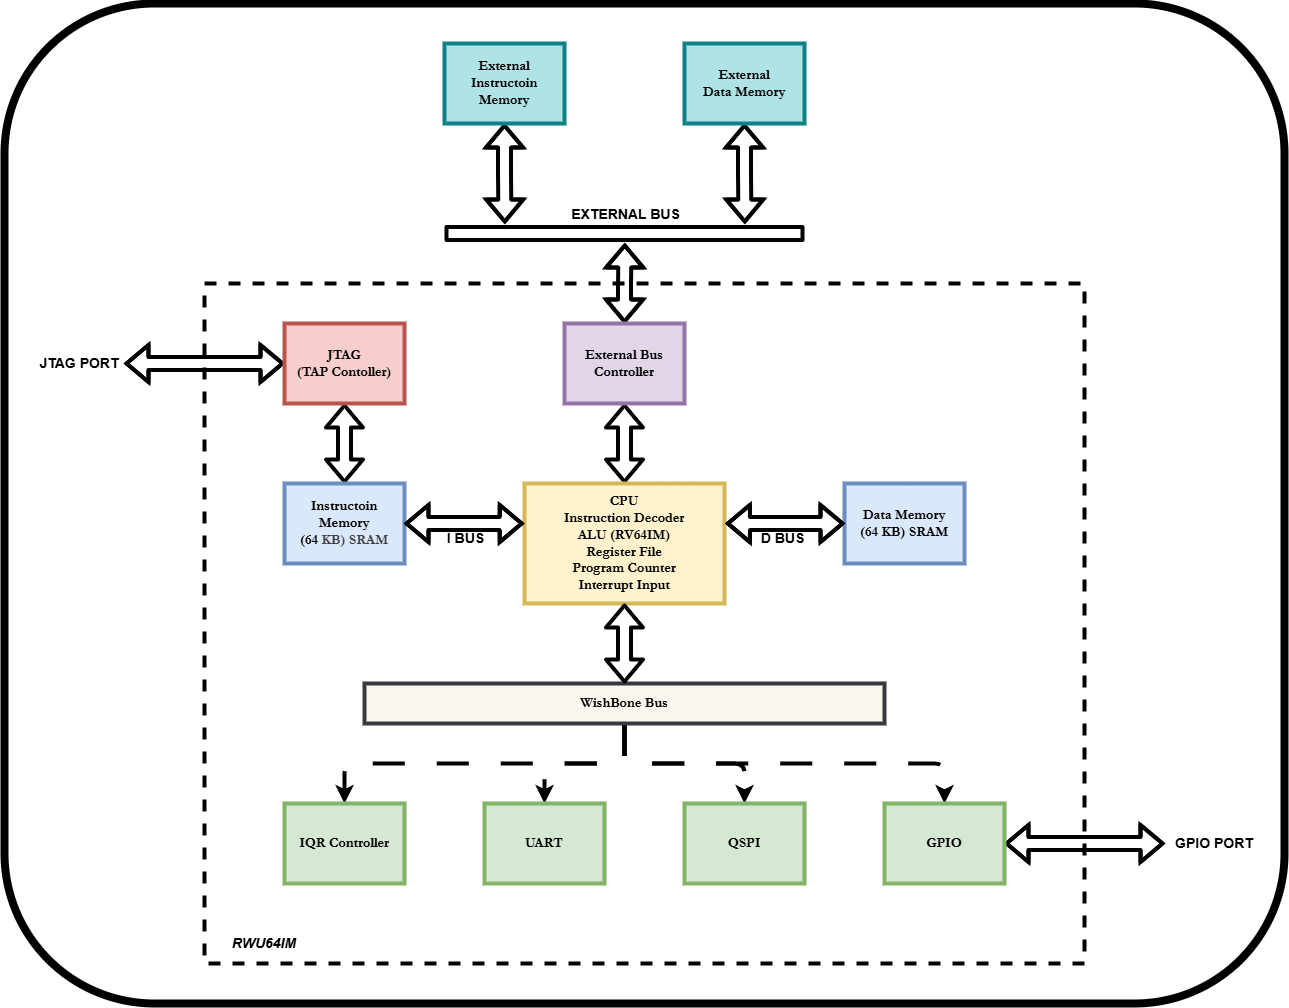
\includegraphics[width=0.9\textwidth]{figures/block_diagram.png}
   \caption{Top Level  Block Diagram of \gls{rv64i} \gls{SoC}}
   \label{fig:blockdiagram}
\end{figure}

\subsection{Introduction}
The designed microcontroller is a 64-bit \gls{riscv} (\gls{rv64i}) based single-core processor aimed at basic embedded applications. It operates at an internal clock frequency of 80 MHz and provides key interfaces such as \gls{gpio}, \gls{uart}, and \gls{qspi} for communication and JTAG for uploading Program on the controller.
The architecture follows the \gls{Harvard} model with separate instruction and data memories. A Wishbone-based interconnect provides standardized communication between the core and peripherals. The peripheral subsystem includes a configurable \gls{gpio} controller with interrupt capability, a \gls{uart} for serial communication, and a \gls{qspi} interface for high-speed memory or peripheral access.
The system integrates a clock generation block capable of supplying phase-shifted or divided clocks to peripherals, enabling dynamic clock configuration for \gls{pwm} and serial interfaces. Programming and debugging are supported through a JTAG interface.
The interrupt controller supports up to eight sources with programmable trigger modes (rising, falling, both, pulse). The design serves as the foundation for future extensions including cache, DMA, and additional interfaces.

\subsection{Key Features} 
The \gls{riscv} \gls{SoC} microcontroller includes the following key features:
\begin{itemize}

    \item \gls{riscv} \gls{rv64i} \gls{isa}
    \item Single-core, single-\gls{pipeline} processor (scalar, in-order)
    \item \gls{Harvard} architecture with separate \gls{I-MEM} and \gls{D-MEM} (64 KB each)
    \item 80 MHz internal main clock with peripheral clock dividers
    \item Wishbone bus architecture for peripheral connectivity
    \item 32 × 64-bit general-purpose registers (x0–x31) and 64-bit program counter
    \item 8 configurable interrupt lines (\gls{IRQ}[7:0]) with vector-based ISR dispatch
    \item Memory-mapped peripherals for modular extensibility
    \item \gls{uart}, \gls{gpio}, \gls{qspi} interfaces
    \item JTAG for programming and on-chip debug access

\section{Architecture Concepts: Overview}

\subsection{Functional Block Diagram} 

\textcolor{blue}{\textbf{\textit{Functional blocks diagram will be included in the final version of this document.}}}

Figure~\ref{fig:blockdiagram} shows the functional block diagram of the device. The architecture 
consists of a processing subsystem, peripheral subsystem, power management unit, and external 
interface controllers. Each block communicates via a shared system bus.

\subsection{Package}

\textcolor{blue}{\textbf{\textit{Package type and pin configuration details will be provided in the final version of this document.}}}

\section{System View} 

\subsection{Application System Description and Use Cases}
The system is intended for use in low-power embedded applications such as IoT sensors, 
wearables, and smart home devices. A typical system setup includes power management, 
the microcontroller, and external communication modules such as BLE or Wi-Fi. The microcontroller is designed as a compact, easy-to-understand \gls{rv64i}-based system suitable for 
educational purposes, \gls{fpga}-based prototyping, and simple embedded control applications. Its clean 
\gls{Harvard} architecture, small peripheral set, and predictable interrupt behavior make it an ideal 
platform for teaching \gls{cpu} \gls{pipeline} concepts, memory systems, bus architectures, and peripheral 
interface design.
Primary use cases include:
\begin{itemize}
  \item Educational demonstrations of the \gls{riscv} instruction set, \gls{pipeline} execution, and memory-mapped I/O.
  \item \gls{fpga}-based prototyping of embedded systems involving \gls{uart}, \gls{gpio}, or \gls{qspi} communication.
  \item Control-oriented applications such as sensor interfacing, simple automation systems, and custom peripherals.
  \item Research or coursework involving modification of the \gls{cpu} \gls{pipeline}, interrupt controller behavior, or clocking subsystem.
\end{itemize}

\subsection{System Description}
The system is organized as a \gls{Harvard}-architecture microcontroller with separate instruction and data memories, unified through a Wishbone interconnect for all data accesses. The \gls{cpu} implements the \gls{rv64i} \gls{isa}and features a straightforward single-\gls{pipeline} structure. The instruction memory (\gls{I-MEM}) provides 64\,KB of program space, while the data memory (\gls{D-MEM}) offers an additional 64\,KB region for stack, heap, and global variables.

All peripherals—including \gls{gpio}, \gls{uart}, \gls{qspi}, the interrupt controller, and clock control module—are exposed via a memory-mapped address space connected through the Wishbone bus. The \gls{cpu} uses standard Wishbone read/write cycles for peripheral accesses, ensuring low design complexity and full visibility for educational study.

The system operates primarily on the 80\,MHz main clock (CLK\_MAIN). Optional phase-shifted or divided clocks are generated through the Peripheral Clock Generator (PCG) to support \gls{pwm} generation, \gls{uart} baud generation, or time-sensitive external interfaces.

\subsection{System Integration and Application Circuit}

For \gls{fpga} deployments, the system integrates cleanly with minimal external circuitry. Key considerations include:
\begin{itemize}
  \item A stable 80\,MHz clock source or PLL block configured within the \gls{fpga} fabric.
  \item External pins for \gls{uart}, \gls{gpio}, \gls{qspi}, and JTAG made available on \gls{fpga} I/O banks.
  \item Proper pin constraints and I/O standards set according to the \gls{fpga} development board.
  \item Optional external \gls{qspi} flash memory interfaced through the \gls{qspi} lines for program storage or data logging.
  \item Decoupling capacitors on power rails and recommended pull-ups for JTAG lines depending on board design.
\end{itemize}

A typical application circuit includes CLK\_MAIN input, reset circuitry, an external \gls{qspi} flash (optional), and standard \gls{uart} TX/RX connectors.

\subsection{Compliances} 

As the design is intended for \gls{fpga}-based educational and prototype systems, no formal compliance certification is mandated. For deployment in commercial hardware, considerations should include:
\begin{itemize}
  \item Electromagnetic compatibility (EMC) guidelines for digital systems.
  \item ESD protection on external \gls{gpio}, \gls{uart}, and \gls{qspi} pins.
  \item Compliance with RoHS and REACH directives for manufacturing.
  \item Ensuring JTAG and debug interfaces meet IEEE 1149.1 standards.
\end{itemize}

The modular design and clean clocking structure facilitate compliance with common embedded hardware regulations if needed.

\section{Architecture Concepts Overview} 

\subsection{Technology}
The microcontroller is intended for implementation in a modern 90\,nm CMOS technology node. 
This process offers high logic density, low leakage, and excellent performance-per-watt characteristics,
making it suitable for compact embedded microcontrollers and \gls{SoC}-class designs. The design targets \gls{fpga} prototyping initially, with plans for \gls{asic} fabrication in the future.

\subsection{System Memory Concept}
The microcontroller follows a \gls{Harvard} architecture in which the Instruction Memory (\gls{I-MEM}), 
Data Memory (\gls{D-MEM}), and Register File are all directly connected to the \gls{cpu} core without passing 
through the Wishbone bus. This separation enables parallel instruction fetch and data access, avoids 
structural hazards, and keeps the \gls{pipeline} implementation simple and predictable.

\textbf{Instruction Memory (\gls{I-MEM})} is a 64\,KB block mapped at address range 
0x0000\,0000–0x0000\,FFFF. It is accessed exclusively by the instruction fetch stage of the \gls{cpu} via 
a dedicated instruction interface. Access is read-only from the \gls{cpu} perspective, allowing efficient 
fetch timing and minimizing critical path delays.

\textbf{Data Memory (\gls{D-MEM})} is a separate 64\,KB block mapped at address range 
0x0001\,0000–0x0001\,FFFF. The \gls{cpu} accesses \gls{D-MEM} through a dedicated data interface that supports 
load and store operations without involving any bus arbitration. Since \gls{D-MEM} is not part of the 
Wishbone interconnect, data operations occur with deterministic timing independent of peripheral 
traffic.

\textbf{The Register File} consists of 32 general-purpose 64-bit registers (x0–x31) and is implemented 
inside the \gls{cpu} core. It provides two read ports and one write port to support single-issue \gls{pipeline} 
operation. The Register File is not memory-mapped and cannot be accessed by peripherals or external 
masters.

\textbf{Peripheral Memory Space} is accessed through the Wishbone bus and is distinct from both \gls{I-MEM} 
and \gls{D-MEM}. Only load/store instructions targeting the high address region (starting at 0x1000\,0000) 
generate Wishbone transactions. This clean separation ensures that:
\begin{itemize}
  \item program execution (\gls{I-MEM}) never competes with data accesses,
  \item core data accesses (\gls{D-MEM}) are unaffected by peripheral latency,
  \item Wishbone traffic originates only from memory-mapped I/O operations.
\end{itemize}

\subsection{Software Architecture}
The software architecture of the microcontroller is based on a conventional \gls{riscv} bare-metal 
development flow. The hardware is implemented and verified using SystemVerilog, while Vivado is used 
as the primary environment for simulation, synthesis, and \gls{fpga} deployment.

Application development is performed using a \gls{riscv} GCC toolchain configured for the \gls{rv64i} \gls{isa}. 
Programs are written in C or assembly and compiled into machine code through the following steps:
\begin{enumerate}
  \item C source files are compiled by the \gls{riscv} compiler into assembly.
  \item The assembler and linker generate a flat binary image targeting the \gls{I-MEM} address map.
  \item A custom programming tool converts the binary into a JTAG-compatible format.
  \item Using the JTAG interface, the tool loads the program directly into the Instruction Memory 
        implemented on the \gls{fpga}.
\end{enumerate}

The microcontroller operates without an operating system, using a simple bare-metal startup sequence 
that initializes the stack pointer, configures peripherals, and optionally enables interrupts. All 
peripherals (\gls{gpio}, \gls{uart}, \gls{qspi}, clock controller, and \gls{IRQ} controller) are controlled using 
memory-mapped register access within the high-address I/O region. The interrupt architecture supports 
hardware-vectored entry, simplifying handler development and reducing interrupt latency.

\subsection{Interprocessor Communication Concept} 

The current microcontroller is a single-core \gls{rv64i} design and therefore does not implement any 
interprocessor communication (IPC) mechanisms. All computation, memory access, and interrupt handling 
occur within the single \gls{cpu} \gls{pipeline}. 

\section{Functional Block Overview}
The microcontroller consists of a compact set of functional modules designed around a clean \gls{Harvard} 
architecture and a Wishbone-based peripheral subsystem. The major functional blocks include:

\begin{itemize}
  \item \textbf{\gls{cpu} Core (\gls{rv64i}):}  
        A single-issue scalar \gls{pipeline} implementing the \gls{rv64i} instruction set. Includes the register 
        file, \gls{alu}, multiplication/division unit, instruction decoder, control logic, and interrupt 
        handling interface.

  \item \textbf{Instruction Memory (\gls{I-MEM}):}  
        A 64\,KB program memory directly connected to the \gls{cpu} fetch stage. Stores executable code and 
        reset vectors.

  \item \textbf{Data Memory (\gls{D-MEM}):}  
        A 64\,KB data RAM directly accessed by the \gls{cpu} load/store unit, supporting low-latency memory 
        operations independent of peripheral traffic.

  \item \textbf{Wishbone Interconnect:}  
        A simple single-master bus used by the \gls{cpu} to access all memory-mapped peripherals. Ensures 
        modular peripheral integration and predictable transaction behavior.

  \item \textbf{\gls{gpio} Controller:}  
        Provides general-purpose digital I/O pins with configurable direction and interrupt capability. 
        Supports optional \gls{pwm} via peripheral clock division.

  \item \textbf{\gls{uart} Controller:}  
        Implements asynchronous serial communication with programmable baud rate and interrupt-driven 
        transmit/receive support.

  \item \textbf{\gls{qspi} Controller:}  
        Provides quad-SPI communication for external flash or high-speed serial devices.

  \item \textbf{Interrupt Controller:}  
        Supports eight individually configurable external interrupt lines with level, edge, and pulse 
        triggering. Generates hardware vector addresses to accelerate ISR entry.

  \item \textbf{Peripheral Clock Generator (PCG):}  
        Generates divided and phase-adjusted clock signals derived from the 80\,MHz main clock for use 
        by \gls{uart}, \gls{gpio} timers, \gls{qspi}, and other peripherals.

  \item \textbf{JTAG Interface:}  
        Enables programming and debugging through a standard IEEE 1149.1–compatible interface.
\end{itemize}

Each module is memory-mapped in the high-address region and integrated through the Wishbone bus, 
while the \gls{cpu}, Register File, \gls{I-MEM}, and \gls{D-MEM} remain directly connected as part of the \gls{Harvard} 
core architecture.


\section{Pin List} 
External pins for the microcontroller include:

\begin{itemize}
  \item \textbf{CLK\_MAIN} – Primary 80\,MHz system clock input.
  \item \textbf{RESET\_N} – System reset, active low.
  \item \textbf{\gls{gpio}[x]} – General-purpose digital input/output pins; each configurable for direction and interrupt triggering.
  \item \textbf{\gls{uart}\_TX, \gls{uart}\_RX} – \gls{uart} communication pins.
  \item \textbf{\gls{qspi}\_SCLK, \gls{qspi}\_CS, \gls{qspi}\_IO[3:0]} – Quad-SPI interface for external flash memory.
  \item \textbf{\gls{IRQ}[7:0]} – External interrupt request inputs.
  \item \textbf{JTAG\_TCK, JTAG\_TMS, JTAG\_TDI, JTAG\_TDO, JTAG\_TRST} – Debug/programming pins.
\end{itemize}

\textcolor{blue}{\textbf{\textit{Pin configuration, multiplexing options, and detailed signal descriptions will be provided in the final revision of this document.}}}

\end{itemize}
